\documentclass{article}
\usepackage[utf8]{inputenc}
\usepackage{graphicx}
\usepackage{gensymb}
\usepackage{textcomp}
\usepackage{hyperref}
\usepackage{parskip}
\usepackage{commath}
\usepackage{float}
\usepackage{cite}
\usepackage{doi}
\graphicspath{ {./images/} }
\usepackage{hyperref}
%
\makeatletter
\setlength{\@fptop}{0pt}
\makeatother
%
\usepackage{geometry}
\usepackage{amsmath}
\usepackage{amsthm}
\usepackage{amsfonts}
\usepackage{ upgreek }
\usepackage[affil-it]{authblk}
\usepackage[export]{adjustbox}
\newtheorem{theorem}{Theorem}[section]
\newtheorem{corollary}{Corollary}[theorem]
\newtheorem{claim}{Claim}
\usepackage{subfigure}
 
\title{Generating Kepler Triangles and Logarithmic Spiral with Recurrent Functions}
\author{Rahul Gohil}
\affil{Student, B.E(Computer Engineering), Thadomal Shahani Engineering College, Mumbai, India}

\date{\vspace{-5ex}}

\providecommand{\keywords}[1]{\textbf{\textit{Keywords ---}} #1}
\begin{document}

\maketitle
\begin{center}
	\href{mailto:rahul.gohil@thadomal.org}{rahul.gohil@thadomal.org}
\end{center}

\begin{abstract}
This paper presents some recurrent functions which we can use to make Kepler Triangles and through their special arrangement we can obtain logarithmic spirals, we also obtain a way get their discrete form.     
\end{abstract}

\keywords{Kepler Triangles, Logarithmic Spirals, Recurrent Functions}

\section{Introduction}
G. Anatriello, G. Vincenzi\cite{paper1} discussed about continue triangles and how they discretize a logarithmic spiral by polygon chains and obtained different discrete spirals known as $(r, k)$-male spirals which discretize well known logarithmic spirals. Here we give a different approach for discretization of logarithmic spiral using kepler triangles. 
\subsection{Defining the Recurrent Function}
Let's take the Fibonacci sequence, $f'(n) = f'(n - 1) + f'(n - 2)$, where $f'(0) = 0$ \& $f'(1) = 1$.\\
It's easy to see that for $A  = \begin{bmatrix}1 & 1 \\ 1 & 0 \end{bmatrix}$ $$A^n = \begin{bmatrix}f'(n + 1) & f'(n) \\ f'(n) & f'(n - 1)\end{bmatrix}$$
Binet's formula for nth Fibonacci number is $f'(n) = \dfrac{\varphi^n - \psi^n}{\sqrt{5}}$, where $\varphi = \dfrac{1 + \sqrt{5}}{2}$ and $\psi = \dfrac{1 - \sqrt{5}}{2}$\cite{BF-wiki}.\\
$\psi = 1 - \varphi = \dfrac{-1}{\varphi}$, therefore Binet's formula can also be written as 
$f'(n) = \dfrac{\varphi^{2n} - (-1)^n}{\varphi^n\sqrt{5}}$\\
Let's take a function \(f\) where $f(n) = \sqrt{f(n - 1)^2 + f(n - 2)^2}$, \(f(0) < f(1)\) and $f(0), f(1) \in \mathbb{R}^{+}$.\\
We can define this sequence in matrix form as
\begin{align*}
\begin{bmatrix}f(n)^2 \\f(n - 1)^2\end{bmatrix} 
&=
\begin{bmatrix}1 & 1\\1 & 0\end{bmatrix}
\begin{bmatrix}f(n - 1)^2\\f(n - 2)^2\end{bmatrix} \\\\
&= \begin{bmatrix}1 & 1 \\1 & 0\end{bmatrix}^{\!n - 1}
\begin{bmatrix}f(1)^2\\f(0)^2\end{bmatrix}\\\\
&= A^{\!n - 1}\begin{bmatrix}f(1)^2\\f(0)^2\end{bmatrix}\\\\
\begin{bmatrix}f(n)^2 \\f(n - 1)^2\end{bmatrix}
&= \begin{bmatrix}f'(n) & f'(n - 1) \\ f'(n - 1) & f'(n - 2)\end{bmatrix}
\begin{bmatrix}f(1)^2 \\f(0)^2\end{bmatrix}\\
\end{align*}
Therefore, $f(n) = \sqrt{f'(n)f(1)^2 + f'(n - 1)f(0)^2}$
\begin{theorem}
	\label{lim-cons}
$$\lim_{n \to \infty} \dfrac{f(n + a)}{f(n + b)} = \varphi^{\left (\displaystyle \frac{a - b}{2} \right)}$$
\end{theorem}
\begin{proof}
\begin{align*}
    \dfrac{f(n + a)}{f(n + b)} &= \dfrac{\sqrt{f(n + a -1)^2 + f(n + a - 2)^2}}{\sqrt{f(n + b - 1)^2 + f(n + b - 2)^2}}\\\\
    &= \dfrac{\sqrt{f'(n + a)f(1)^2 + f'(n + a - 1)f(0)^2}}{\sqrt{f'(n + b)f(1)^2 + f'(n + b - 1)f(0)^2}}\\\\
    &= \dfrac{\sqrt{f'(n + a - 1)\left(\dfrac{f'(n + a)f(1)^2}{f'(n + a - 1)} + f(0)^2\right)}}{\sqrt{f'(n + b - 1)\left(\dfrac{f'(n + b)f(1)^2}{f'(n + b - 1)} + f(0)^2\right)}}\\\\
    &= \dfrac{\sqrt{\dfrac{\varphi^{2(n + a)} - (-1)^{n + a}}{\varphi^{n + a}\sqrt{5}}\left(\dfrac{f'(n + a)f(1)^2}{f'(n + a - 1)} + f(0)^2\right)}}{\sqrt{\dfrac{\varphi^{2(n + b)} - (-1)^{n + b}}{\varphi^{n + b}\sqrt{5}}\left(\dfrac{f'(n + b)f(1)^2}{f'(n + b - 1)} + f(0)^2\right)}}\\\\
    \lim_{n \to \infty} \dfrac{f(n + a)}{f(n + b)}
    &= \lim_{n \to \infty} \dfrac{\sqrt{\dfrac{\varphi^{2(n + a)} - (-1)^{n + a}}{\varphi^{n + a}\sqrt{5}}\left(\dfrac{f'(n + a)f(1)^2}{f'(n + a - 1)} + f(0)^2\right)}}{\sqrt{\dfrac{\varphi^{2(n + b)} - (-1)^{n + b}}{\varphi^{n + b}\sqrt{5}}\left(\dfrac{f'(n + b)f(1)^2}{f'(n + b - 1)} + f(0)^2\right)}}\\\\
    &= \dfrac{\sqrt{\dfrac{\varphi^{2(n + a)}}{\varphi^{n + a}}\left(\varphi f(1)^2 + f(0)^2\right)}}{\sqrt{\dfrac{\varphi^{2(n + b)}}{\varphi^{n + b}}\left(\varphi f(1)^2 + f(0)^2\right)}}\\\\
    &= \sqrt{\varphi^{2(n + a) - n - a - 2(n + b) + n + b}}\\
    &= \sqrt{\varphi^{2n + 2a - n - a -2n -2b + n + b}}\\
    \lim_{n \to \infty} \dfrac{f(n + a)}{f(n + b)}
    &= \varphi^{\left (\displaystyle \frac{a - b}{2} \right)}
\end{align*}
\end{proof}
\subsection{Geometric Interpretation}
\label{geo}
The function $f(n)$ can be geometrically defined as length of a hypotenuse of a triangle whose base has length $f(n - 2)$ and height of length $f(n - 1)$. Now if we assume a line perpendicular to line $B_1B_2$ in Figure 1 at \ref{fig1} passing through point $B_2$ and mark a point at length $f(n)$ from $B_2$ we get $B_3$ and then connect $B_1$ and $B_3$ we get it's length to be $f(n + 1)$. Similarly we can generate more points, lines and triangles using this method.\\ Let $(x_1, y_1)$ be any point on the 2D Plane, $x_1 < f(0)$, $y_1 < f(1)$. Let $(f(0) + x_1, y_1)$ and $(f(0) + x_1, f(1) + y_1)$ be points on the plane, by connecting them we get the triangle illustrated in Figure 2 at \ref{fig1} which has it's length of hypotenuse as $f(2)$.\\
\begin{figure}
    \centering
    \begin{minipage}{0.45\textwidth}
    	\label{fig1}
        \centering
        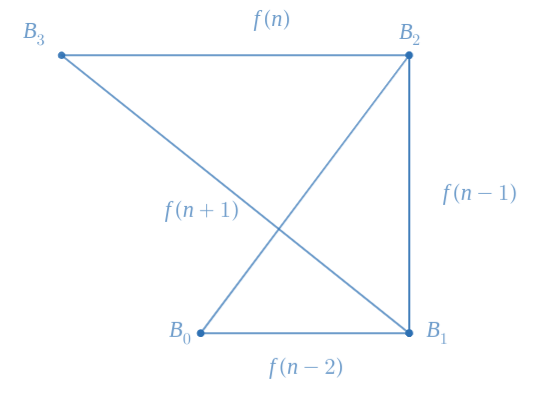
\includegraphics[scale=0.4]{images/GFKT1.png}
        \caption{nth and (n+1)th triangle}
    \end{minipage}\hfill
    \begin{minipage}{0.45\textwidth}
        \centering
        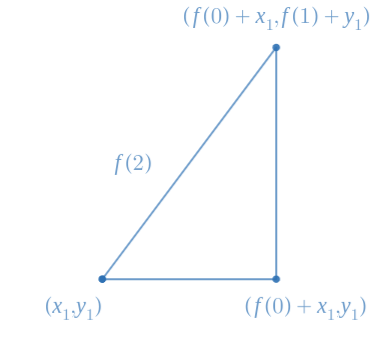
\includegraphics[scale=0.46]{images/GFKT2.png}
        \caption{Initial Triangle}
    \end{minipage}
\end{figure}
Let $I_0 = (x_1, y_1)$ and $I_1 = (f(0) + x_1, y_1)$, we define a function $P$ which is point on the 2D Plane.\\
Let $P(0) = (f(0) + x_1, f(1) + y_1)$, the $P$ function has 2 class variables(a class variable is used to denote a variable associated with the object of that class in programming languages), namely $x$ and $y$, which denote the x co-ordinate and y co-ordinate of that point respectively.\\
We define $P(n)$ as
\begin{equation*}
    P(n) = \begin{cases}
            (P(n - 1).x - f(n + 1), P(n - 1).y) & n \equiv 1\mod 4\\
            (P(n - 1).x, P(n - 1).y - f(n + 1)) & n \equiv 2\mod 4\\
            (P(n - 1).x + f(n + 1), P(n - 1).y) & n \equiv 3\mod 4\\
            (P(n - 1).x, P(n - 1).y + f(n + 1)) & n \equiv 0\mod 4
            \end{cases}
\end{equation*}
We define a function $L$ which is a line on the 2D Plane.\\
Let $L(0) = (I_0, P(0))$, this means that $L(0)$ is a line between points $I_0$ and $P(0)$, $L(1) = (I_1, P(1))$. $L$ function has 5 class variables, namely $point1$, $point2$, $slope$, $constant$, $length$ denoting the first point in the tuple, the second point in the tuple, slope of the line, the constant associated with it and the length of the line respectively.\\
We define $L(n)$ as $$L(n) = (L(n - 2).point2, P(n))$$ 
Essentially $L(n)$ is the hypotenuse of the nth triangle.
We also define a function $L'$ which describes base and height of a triangle which has same class variables as $L$.
Let $L'(0) = (I_0, I_1)$ and $L'(1) = (I_1, P(0))$.
$$L'(n) = (L'(n - 1).point2, P(n - 1))$$
Let's also define a function for a triangle $T$, $T(0) = (L'(0), L'(1), L(0))$. $T$ function has 3 class variables $line1$, $line2$ and $line3$, denoting base, height and hypotenuse respectively.
$$T(n) = (T(n - 1).line2, L'(n + 1), L(n))$$
For each $n$, $L'(n)$ is the base, $L'(n + 1)$ is the height and $L(n)$ is the hypotenuse of triangle $T(n)$.\\
Through out this paper, we are going to assume $n$ being an integer such that $n \equiv 0\mod4$
\begin{theorem}
	\label{lim-P}
$$\lim_{n \to \infty} P(n).x - x_1 = f(n - 2)$$
\end{theorem}
\begin{proof}
$P(n).x$ can alternatively be defined as $$P(n).x = x_1 + \sum_{i = 0}^{n / 2}(-1)^i f(2i)$$.
$$P(n).x - x_1 = \sum_{i = 0}^{n / 2}(-1)^i f(2i)$$
Let $g(n) = \dfrac{P(n).x - x_1}{f(n - 2)} - 1$
\begin{align*}
    g(n) &= \dfrac{\displaystyle\sum_{i = 0}^{n / 2}(-1)^i f(2i)}{f(n - 2)} - 1\\
    &= \sum_{i = 0}^{n / 2}\dfrac{(-1)^i f(2i)}{f(n - 2)} - 1\\
    \text{Using \ref{lim-cons}}\\
    g(n) &= \sum_{i = 0}^{n / 2}(-1)^i \varphi^{(\frac{2i - n + 2}{2})}- 1
\end{align*}
Let $S(n) = \displaystyle\sum_{i = 0}^{n/2}(-1)^i \varphi^{(\frac{2i-n+2}{2})}$\\
The terms of $S(n)$ are $\varphi^{(\frac{-(n - 2)}{2})} - \ldots + \varphi^{-3} - \varphi^{-2} + \varphi^{-1} -\varphi^0 + \varphi$.\\
Therefore $S(n)$ can also be defined as $$S(n) = \sum_{i = 0}^{n / 2}(-1)^i \varphi^{1 - i}$$
\begin{claim}
	\begin{equation*}
	S(n) = \begin{cases}
	f'(n + 1)\varphi^{-n} + (f'(n) + 1)\varphi^{-n-1} & n\equiv0\mod4\hspace{2mm} or\hspace{2mm} n\equiv2\mod4\\
	f'(n + 1)\varphi^{-n} + (f'(n) - 1)\varphi^{-n-1} &
	n\equiv1\mod4\hspace{2mm} or\hspace{2mm} n\equiv3\mod4
	\end{cases}
	\end{equation*}
\end{claim}
\begin{proof}
	Let's prove this by mathematical induction.\\
	Base Case $n=0$, $S(n) = \varphi$ is our left side, $f'(0 + 1)\varphi^0 + (f'(0) + 1)\varphi^{-1} = 1 + \varphi^{-1}$ is our right side.\\
	Using the formula $\varphi^n = \varphi^{n - 1} + \varphi^{n - 2}$\cite{PowerP}, right side can be written as $\varphi^0 + \varphi^{-1} = \varphi$, which is equal to left side.\\
	So the theorem holds for $n = 0$\\
	Inductive hypothesis : Suppose the proposition holds for all values of $n$ upto some $k$, $k \geq 1$\\
	Inductive step : Let $n = k + 1$, and $k \equiv0\mod4$ then our left side is,
	\begin{align*}
	S(k + 1) &= f'(k+2)\varphi^{-k-1} + (f'(k+1)-1)\varphi^{-k-2}\\
	\end{align*}
	Our right side is,
	\begin{align*}
		S(k + 1) &= \varphi - \varphi^0 + \varphi^{-1} - \ldots + \varphi^{1 - k} - \varphi^{1 - (k + 1)}\\
		&= f'(k + 1)\varphi^{-k} + (f'(k) + 1)\varphi^{-k-1} - \varphi^{-k}\\
		&= f'(k + 1)\varphi^{-k-1} + f'(k+1)\varphi^{-k-2}+f'(k)\varphi^{-k-1}+\varphi^{-k-1}-\varphi^{-k}\\
		S(k + 1) &= f'(k+2)\varphi^{-k-1} + (f'(k+1)-1)\varphi^{-k-2}
	\end{align*}
	Since $f'(k+2) = f'(k+1)+f'(k)$ and $\varphi^{-k} = \varphi^{-k-1}+\varphi^{-k-2}$,
	which is our left side.\\
	So the theorem holds for $n = k + 1$, therefore by the principle of mathematical induction, the theorem holds for all $n \in \mathbb{N}$
\end{proof}
$$g(n) = S(n) - 1$$
\begin{align*}
	S(n) &= f'(n+1)\varphi^{-n} + (f'(n) + 1)\varphi^{-n-1}\\
	&= f'(n+1)\varphi^{-n}+f'(n)^{-n-1}+\varphi^{-n-1}\\\\
	&= \dfrac{\varphi^{2(n+1)}-(-1)^{n+1}}{\varphi^{n+1}\sqrt{5}\hspace{1mm}\varphi^n} + \dfrac{\varphi^{2(n)}-(-1)^{n}}{\varphi^{n}\sqrt{5}\hspace{1mm}\varphi^{n+1}} + \varphi^{-n-1}\\\\
	&= \dfrac{\varphi^{2(n+1)}+\varphi^{2n}}{\varphi^{2n+1}\sqrt{5}}+ \varphi^{-n-1}\\\\
	&= \dfrac{\varphi^{2n}(\varphi^2+1)}{\varphi^{2n+1}\sqrt{5}}+\varphi^{-n-1}\\\\
	&=\dfrac{\varphi^2+1}{\varphi\sqrt{5}}+\varphi^{-n-1}\\
	&= \dfrac{5+\sqrt{5}}{\varphi\hspace{1mm}2\sqrt{5}}+\varphi^{-n-1}\\
	&= \dfrac{1+\sqrt{5}}{2\varphi}+\varphi^{-n-1}\\
	S(n) &= 1 + \varphi^{-n-1}\\
	\lim_{n \to \infty} S(n) &= 1\\
	\lim_{n \to \infty} g(n) &= \lim_{n \to \infty} S(n) - 1\\
	\lim_{n \to \infty} g(n) &= 0\\
\end{align*}
\begin{align*}
	&\lim_{n \to \infty} \dfrac{P(n).x - x_1}{f(n - 2)} - 1 = 0\\
	&\lim_{n \to \infty} \dfrac{P(n).x - x_1}{f(n - 2)} = 1\\
	&\lim_{n \to \infty} P(n).x -x_1 = f(n-2)
\end{align*}
\end{proof}
Similarly we can prove that,
\begin{align*}
	&\lim_{n \to \infty} P(n).y -y_1 = f(n-1)\\
	&\lim_{n \to \infty} P(n+1).x -x_1 = -f(n)
\end{align*}
\begin{theorem}
	\label{lim-angle}
	As $n \to \infty$, angle between $L(n)$ and $L(n+1)$ tends $\to 90^\circ$
\end{theorem}
\begin{proof}
	Let $A(n)$ be angle between $L(n)$ and $L(n+1)$
	$$A(n) = \tan^{-1}\left({\abs{\dfrac{L(n+1).slope-L(n).slope}{1+(L(n+1).slope \cdot L(n).slope)}}}\right)$$
	Let $1 + (L(n+1).slope \cdot L(n).slope) = a$\\
	$L(n+1) = (P(n-1), P(n+1))$ and $L(n) = (P(n-2), P(n))$
	\begin{align*}
		L(n+1).slope &= \dfrac{a - 1}{L(n).slope}\\
		\dfrac{P(n+1).y - P(n-1).y}{P(n+1).x - P(n-1).x} &= \dfrac{(a-1)(P(n).x-P(n-2).x)}{P(n).y-P(n-2).y}
	\end{align*}
	$P(n+1) = (P(n).x - f(n+2), P(n).y)$\\
	$P(n) = (P(n-1).x, P(n-1).y+f(n+1))$\\
	$P(n-1) = (P(n-2).x+f(n), P(n-2).y)$
	\begin{align*}
		\dfrac{P(n).y-P(n-2).y}{P(n).x-P(n-2).x-f(n+2)-f(n)} &= \dfrac{(a-1)(P(n).x-P(n-2).x)}{P(n).y-P(n-2).y}
	\end{align*}
	$P(n).x = P(n-1).x = P(n-2).x+f(n)$, therefore $P(n).x-P(n-2).x=f(n)$\\
	$P(n.y) = P(n-1).y+f(n-1)$ and $P(n-1).y = P(n-2).y$, therefore $P(n).y-P(n-2)=f(n+1)$
	\begin{align*}
		\dfrac{f(n+1)}{f(n)-f(n+2)-f(n)} &= \dfrac{(a-1)(f(n))}{f(n+1)}\\
		\dfrac{-f(n+1)^2}{f(n+2)f(n)} &= a - 1
	\end{align*}
	Let $g'(n) = \dfrac{-f(n+1)^2}{f(n+2)f(n)}$, using \ref{lim-cons},
	$$\lim_{n \to \infty}g'(n) = \dfrac{-\sqrt{\varphi}}{\sqrt{\varphi}}$$
	$$\lim_{n \to \infty}g'(n) = -1$$
	$$\lim_{n \to \infty}g'(n) = a - 1$$
	$$-1 = a - 1$$
	$$a = 0$$
	Therefore, $$\lim_{n \to \infty}1 + (L(n+1).slope \cdot L(n).slope) = 0$$
	Since, $\tan^{-1}{\dfrac{1}{0}} = 90^\circ$
	$$\lim_{n \to \infty} A(n) = 90^\circ$$
	Therefore, as $n \to \infty$, angle between $L(n)$ and $L(n+1)$ tends $\to 90^\circ$
\end{proof}
\begin{theorem}
	As $n \to \infty$, $P(n+2)$ tends to satisfy $L(n)$
\end{theorem}
\begin{proof}
	Let's satisfy $P(n+2)$ in $L(n)$ equation.
	$$S'(n) = P(n+2).y - L(n).slope \cdot P(n+2).x - L(n).constant$$
	$L(n) = (P(n-2), P(n))$\\
	$L(n).slope = \dfrac{P(n).y-P(n-2).y}{P(n).x-P(n-2).x} = \dfrac{f(n+1)}{f(n)}$ as seen in \ref{lim-angle}\\
	$L(n).constant = P(n).y - L(n).slope \cdot P(n).x = P(n).y - \dfrac{f(n+1)}{f(n)} P(n).x$\\
	$P(n+2) = (P(n+1).x, P(n+1).y-f(n+3))$\\
	$P(n+1) = (P(n).x - f(n+2), P(n).y)$
	\begin{align*}
		S'(n) &= P(n).y - f(n+3)-\dfrac{f(n+1)}{f(n)}(P(n).x-f(n+2))-\left(P(n).y-\dfrac{f(n+1)}{f(n)}P(n).x\right)\\
		&= \dfrac{f(n+2)f(n+1)}{f(n)}-f(n+3)\\
		&= \dfrac{f(n+2)f(n+1)}{f(n)}-\dfrac{f(n+3)f(n+2)}{f(n+2)}
	\end{align*}
	Using \ref{lim-cons}
	\begin{align*}
		&\lim_{n \to \infty} S'(n) = \sqrt{\varphi}f(n+2) - \sqrt{\varphi}f(n+2)\\
		&\lim_{n \to \infty} S'(n) = 0
	\end{align*}
	Therefore, as $n\to\infty$, $P(n+2)$ tends to satisfy $L(n)$
\end{proof}
\begin{corollary}
	As $n \to \infty$, all $P(n)$ with even $n$ tend to lie on the same line, same is true for all $P(n)$ with odd $n$.
\end{corollary}
\begin{proof}
	$L(n) = (P(n-2), P(n))$, therefore, for some $n$, $(P(n-2), P(n), P(n+2))$, all lie on the same line.\\
	Similarly $P(n+4)$ satisfies $L(n+2)$, where $(P(n), P(n+2), P(n+4))$ lie on the same line. Since $P(n-2)$ and $P(n)$ lie on the same line, $P(n-2)$ and $P(n+4)$ must lie on the same line.\\
	Therefore $$(\ldots, P(n-2), P(n), P(n+2), P(n+4),\ldots)$$ lie on the same line.
\end{proof}

\section{Generating Kepler Triangles}
A Kepler triangle is a right angled triangle whose edge-lengths are in geometric progression with $\sqrt{\varphi}$ as the common ratio and can be written as 1 : $\sqrt{\varphi}$ : $\varphi$\cite{KT-wiki}.
\begin{theorem}
	As $n \to \infty$, $T(n)$ is a kepler triangle.
\end{theorem}
\begin{proof}
	$T(n) = (T(n-1).line2, L'(n+1), L(n))$\\
	$T(n-1) = (T(n-2).line2, L'(n), L(n))$\\
	Therefore, $T(n) = (L'(n), L'(n+1), L(n))$
	\begin{align*}
		\dfrac{L'(n+1).length}{L'(n).length} &= \dfrac{\sqrt{(P(n).x - P(n-1).x)^2 + (P(n).y-P(n-1).y)^2}}{\sqrt{(P(n-1).x - P(n-2).x)^2 + (P(n-1).y-P(n-2).y)^2}}\\
		\dfrac{L'(n+1).length}{L'(n).length} &= \dfrac{f(n+1)}{f(n)}
	\end{align*}
	Using \ref{lim-cons}
	$$\lim_{n \to \infty} \dfrac{L'(n+1).length}{L'(n).length} = \sqrt{\varphi}$$
	\begin{align*}
	\dfrac{L(n).length}{L'(n).length} &= \dfrac{\sqrt{(P(n).x - P(n-2).x)^2 + (P(n).y-P(n-2).y)^2}}{\sqrt{(P(n-1).x - P(n-2).x)^2 + (P(n-1).y-P(n-2).y)^2}}\\
	\dfrac{L(n).length}{L'(n).length} &= \dfrac{f(n+2)}{f(n)}
	\end{align*}
	Using \ref{lim-cons}
	$$\lim_{n \to \infty} \dfrac{L(n).length}{L'(n).length} = \varphi$$
	Therefore, as $n \to \infty$
	$$\dfrac{L'(n).length}{L'(n).length} : \dfrac{L'(n+1).length}{L'(n).length} : \dfrac{L(n).length}{L'(n).length} = 1 : \sqrt{\varphi} : \varphi $$
	Therefore, as $n \to \infty$, $T(n)$ is a kepler triangle.
\end{proof}
\begin{corollary}
	As $n \to \infty$, $T(n)$ is similar to $T(n+1)$
\end{corollary}
\begin{proof}
	Since both $T(n)$ and $T(n+1)$ are kepler triangles, when we scale $T(n)$ by $\sqrt{\varphi}$ we get $T(n+1)$ or use \ref{lim-angle} and use SAS test.
\end{proof}
\section{Logarithmic Spiral}
Equation of a logarithmic spiral in polar form is,
{\large $$r = ae^{k\theta}$$}
where $a$ and $k$ are constants\cite{LS-wiki}.\\
To determine $a$ and $k$, consider the equations,
{\large$$r_n = ae^{k\theta_n}$$}
{\large$$r_{n+1}=ae^{k\theta_{n+1}}$$}
{\large $\theta_n$} can be defined as,
\begin{equation*}
	 \theta_n = \begin{cases}
		\lfloor\frac{n}{4}\rfloor 2\pi + \tan^{-1}({L(I_0, P(n)).slope}) & n\equiv0\mod4\\
		\lfloor\frac{n}{4}\rfloor 2\pi + \tan^{-1}({L(I_0, P(n)).slope}) + \pi & n\equiv 1 \mod4 \hspace{2mm}or\hspace{2mm} n\equiv 2\mod4\\
		\lfloor\frac{n}{4}\rfloor 2\pi + \tan^{-1}({L(I_0, P(n)).slope}) + 2\pi & n\equiv3\mod4
	\end{cases}
\end{equation*}
where $L(I_0, P(n))$ is a line which passes through $I_0$ and $P(n)$.\\
{\large $r_n$} can be defined as,
$$r_n = \sqrt{(P(n).x -x_1)^2 + (P(n).y - y_1)^2}$$
Now,
\begin{align*}
	 \dfrac{r_{n+1}}{r_n} &= e^{k(\theta_{n+1}-\theta_n)}\\
	 k &= \dfrac{\ln{\left(\dfrac{r_{n+1}}{r_n}\right)}}{\theta_{n+1}-\theta_n}\\
	 &= \dfrac{\ln{\left(\dfrac{\sqrt{(P(n+1).x -x_1)^2 + (P(n+1).y - y_1)^2}}{\sqrt{(P(n).x -x_1)^2 + (P(n).y - y_1)^2}}\right)}}{\lfloor\frac{n+1}{4}\rfloor 2\pi + \tan^{-1}({L(I_0, P(n+1)).slope}) + \pi -\lfloor\frac{n}{4}\rfloor 2\pi - \tan^{-1}({L(I_0, P(n)).slope})}\\\\
	 &= \dfrac{\ln{\left(\dfrac{\sqrt{(P(n+1).x -x_1)^2 + (P(n).y - y_1)^2}}{\sqrt{(P(n).x -x_1)^2 + (P(n).y - y_1)^2}}\right)}}{\tan^{-1}\left({\dfrac{P(n+1).y - y_1}{P(n+1).x - x_1}}\right) - \tan^{-1}\left({\dfrac{P(n).y - y_1}{P(n).x - x_1}}\right)+ \pi}\\
	 \text{Using \ref{lim-P}}\\
	 \lim_{n \to \infty} k&= \dfrac{\ln{\left(\dfrac{\sqrt{(-f(n))^2 + f(n-1)^2}}{\sqrt{f(n-2)^2 + f(n-1)^2}}\right)}}{\tan^{-1}\left({\dfrac{f(n-1)}{-f(n)}}\right) - \tan^{-1}\left({\dfrac{f(n-1)}{f(n-2)}}\right)+ \pi}\\
	 &= \dfrac{\ln{\left(\dfrac{f(n+1)}{f(n)}\right)}}{\tan^{-1}\left({\dfrac{f(n-1)}{-f(n)}}\right) - \tan^{-1}\left({\dfrac{f(n-1)}{f(n-2)}}\right)+ \pi}\\
	 \text{Using \ref{lim-cons}}\\
	 &= \dfrac{\ln{\left(\sqrt{\varphi}\right)}}
	 {\tan^{-1}\left({\dfrac{-1}{\sqrt{\varphi}}}\right) - \tan^{-1}\left({\sqrt{\varphi}}\right)+ \pi}\\
	 &= \dfrac{\ln{\left(\sqrt{\varphi}\right)}}
	 {-\tan^{-1}\left({\dfrac{1}{\sqrt{\varphi}}}\right) - \tan^{-1}\left({\sqrt{\varphi}}\right)+ \pi}
\end{align*}
\begin{align*}
	&= \dfrac{\ln{\left(\sqrt{\varphi}\right)}}
	{-\tan^{-1}\left({\dfrac{\dfrac{1}{\sqrt{\varphi}}+\varphi}{1 - \dfrac{\sqrt{\varphi}}{\sqrt{\varphi}}}}\right) + \pi}\\
	&= \dfrac{\ln{\left(\sqrt{\varphi}\right)}}{\pi - \dfrac{\pi}{2}}\\
	&= \dfrac{2\ln{\left(\sqrt{\varphi}\right)}}{\pi}\\
	\text{Therefore,}\\
	k &= \dfrac{\ln{\left(\varphi\right)}}{\pi}
\end{align*}
Now, 
	{\large$r = ae^{k\theta} = 
		ae^{\frac{\ln{\varphi}}{\pi}\theta} = a\varphi^{\frac{\theta}{\pi}}$}
\begin{align*}
	a &= r\varphi^{-\dfrac{\theta}{\pi}}\\
	&= r_n\varphi^{-\dfrac{\theta_n}{\pi}}\\
	&= r_n\varphi^{-\left(\dfrac{\lfloor\frac{n}{4}\rfloor2\pi + \tan^{-1}{\left(\dfrac{P(n).y-y_1}{P(n).x - x_1}\right)}}{\pi}\right)}\\
	&= r_n\varphi^{-\left(\dfrac{n}{2} + \dfrac{ \tan^{-1}{\left(\dfrac{P(n).y-y_1}{P(n).x - x_1}\right)}}{\pi}\right)}\\
	&= \dfrac{r_n}{\varphi^{\frac{n}{2}}}\varphi^{-\left(\dfrac{ \tan^{-1}{\left(\dfrac{P(n).y-y_1}{P(n).x - x_1}\right)}}{\pi}\right)}\\
	&= \sqrt{\dfrac{(P(n).x-x_1)^2 + (P(n).y-y_1)^2}{\varphi^n}}\hspace{2mm}\varphi^{-\left(\dfrac{ \tan^{-1}{\left(\dfrac{P(n).y-y_1}{P(n).x - x_1}\right)}}{\pi}\right)}\\
	\text{Using \ref{lim-P}}\\
	&= \sqrt{\dfrac{f(n-2)^2 + f(n-1)^2}{\varphi^n}}\hspace{2mm}\varphi^{-\left(\dfrac{ \tan^{-1}{\left(\dfrac{f(n-1)}{f(n-2)}\right)}}{\pi}\right)}\\
	\text{Using \ref{lim-cons}}\\
	&= \sqrt{\dfrac{f(n-2)^2 (1 + \varphi)}{\varphi^n}}\hspace{2mm}\varphi^{-\left(\dfrac{ \tan^{-1}{\left(\sqrt{\varphi}\right)}}{\pi}\right)}\\
	&= \sqrt{\dfrac{f'(n-2)f(1)^2+f'(n-3)f(0)^2}{\varphi^n}}\hspace{2mm}\sqrt{1+\varphi}\hspace{2mm}\varphi^{-\left(\dfrac{ \tan^{-1}{\left(\sqrt{\varphi}\right)}}{\pi}\right)}
\end{align*}
\begin{align*}
	&= \sqrt{\dfrac{f'(n-3)}{\varphi^n}}\hspace{2mm}\sqrt{(\varphi f(1)^2 + f(0)^2)(1+\varphi)}\hspace{2mm}\varphi^{-\left(\dfrac{ \tan^{-1}{\left(\sqrt{\varphi}\right)}}{\pi}\right)}\\
	&= \sqrt{\dfrac{\varphi^{2(n-3)}-(-1)^{n-3}}{\varphi^{n-3}\sqrt{5}\hspace{1mm}\varphi^n}}\hspace{2mm}\sqrt{(\varphi f(1)^2 + f(0)^2)(1+\varphi)}\hspace{2mm}\varphi^{-\left(\dfrac{ \tan^{-1}{\left(\sqrt{\varphi}\right)}}{\pi}\right)}\\
	&= \sqrt{\dfrac{\varphi^{2n-6}}{\varphi^{2n-3}\sqrt{5}}}\hspace{2mm}\sqrt{(\varphi f(1)^2 + f(0)^2)(1+\varphi)}\hspace{2mm}\varphi^{-\left(\dfrac{ \tan^{-1}{\left(\sqrt{\varphi}\right)}}{\pi}\right)}\\
	a &= \sqrt{\dfrac{(\varphi f(1)^2 + f(0)^2)(1+\varphi)}{\varphi^3\hspace{1mm}\sqrt{5}}}\hspace{2mm}\varphi^{-\left(\dfrac{ \tan^{-1}{\left(\sqrt{\varphi}\right)}}{\pi}\right)}\\
	\text{Therefore,}\\
	a &= \sqrt{\dfrac{\varphi f(1)^2 + f(0)^2}{\varphi\hspace{1mm}\sqrt{5}}}\hspace{2mm}\varphi^{-\left(\dfrac{ \tan^{-1}{\left(\sqrt{\varphi}\right)}}{\pi}\right)}
\end{align*}
Therefore, we obtained the constants $$k = \ln{\dfrac{\varphi}{\pi}} \hspace{2mm}\text{and}\hspace{2mm}a=\sqrt{\dfrac{\varphi f(1)^2 + f(0)^2}{\varphi\hspace{1mm}\sqrt{5}}}\hspace{2mm}\varphi^{-\left(\dfrac{ \tan^{-1}{\left(\sqrt{\varphi}\right)}}{\pi}\right)}$$
The equation of logarithmic spiral is $$r = a\varphi^{\dfrac{\theta}{\pi}}$$
\begin{theorem}
	As $n \to \infty$ $P(n)$ satisfies the logarithmic spiral
\end{theorem}
\begin{proof}
Consider cartesian equation of logarithmic spiral, $$y = r\sin{\theta} \hspace{2mm}\text{and}\hspace{2mm}x = r\cos{\theta}$$
$$y_n = r_n\sin{\theta_n} \hspace{2mm}\text{and}\hspace{2mm}x_n = r_n\cos{\theta_n}$$
$r_n = \sqrt{(P(n).x - x_1)^2 + (P(n).y - y_1)^2}$, using \ref{lim-P} $\lim_{n \to \infty} r_n = f(n)$\\
Let $s = L(I_0, P(n)).slope$
$$\theta_n = \lfloor\dfrac{n}{4}\rfloor 2\pi + \tan^{-1}(L(I_0, P(n)).slope) = \dfrac{n\pi + 2\tan^{-1}(s)}{2}$$
Using the trigonometric relation $2\tan^{-1}(x) = \cos^{-1}\left(\dfrac{1-x^2}{1+x^2}\right)$
$$\theta_n = \dfrac{n\pi + \cos^{-1}\left(\frac{1-s^2}{1+s^2}\right)}{2}$$
Since $s > 1$, $1 - s^2 < 0$, therefore $\cos^{-1}\left(\frac{1-s^2}{1+s^2}\right) = \cos^{-1}\left(\frac{(-1)(s^2-1)}{1+s^2}\right) = \pi - \cos^{-1}\left(\frac{(s^2-1)}{1+s^2}\right)$
$$\theta_n = \dfrac{(n+1)\pi - \cos^{-1}\left(\frac{(s^2-1)}{1+s^2}\right)}{2}$$
$$\sin\theta_n = \sin\left(\dfrac{(n+1)\pi - \cos^{-1}\left(\frac{s^2-1}{1+s^2}\right)}{2}\right)\hspace{2mm}\text{and}\hspace{2mm}\cos\theta_n = \cos\left(\dfrac{(n+1)\pi - \cos^{-1}\left(\frac{s^2-1}{1+s^2}\right)}{2}\right)$$
Using the trignometric relations $\sin\left(\dfrac{x}{2}\right) = \sqrt{\dfrac{1 - \cos(x)}{2}}$ and $\cos\left(\dfrac{x}{2}\right) = \sqrt{\dfrac{1 + \cos(x)}{2}}$
$$\sin\theta_n = \sqrt{\dfrac{1 - \cos\left((n+1)\pi - \cos^{-1}\left(\frac{s^2-1}{1+s^2}\right)\right)}{2}}\hspace{2mm}\text{and}\hspace{2mm}\cos\theta_n = \sqrt{\dfrac{1 + \cos\left((n+1)\pi - \cos^{-1}\left(\frac{s^2-1}{1+s^2}\right)\right)}{2}}$$
Using the trignometric relation $\cos(A-B) = \cos(A)\cos(B)+\sin(A)\sin(B)$
\begin{multline}
	$$\cos\left((n+1)\pi - \cos^{-1}\left(\frac{s^2-1}{1+s^2}\right)\right)=\cos((n+1)\pi)\cos\left(\cos^{-1}\left(\frac{s^2-1}{1+s^2}\right)\right)+\\ \sin((n+1)\pi)\sin\left(\cos^{-1}\left(\frac{s^2-1}{1+s^2}\right)\right)$$
\end{multline}
Using $\cos(n\pi) = (-1)^n\text{and}\sin(n\pi) = 0$, $\cos((n+1)\pi) = (-1)$, $\sin((n+1)\pi) = 0$
\begin{align*}
	\cos\left((n+1)\pi - \cos^{-1}\left(\frac{s^2-1}{1+s^2}\right)\right) &= (-1)\left(\frac{s^2-1}{1+s^2}\right)
\end{align*}
Therefore, $$\sin\theta_n = \sqrt{\dfrac{1 + \left(\frac{s^2-1}{1+s^2}\right)}{2}}\hspace{2mm}\text{and}\hspace{2mm}\cos\theta_n = \sqrt{\dfrac{1 - \left(\frac{s^2-1}{1+s^2}\right)}{2}}$$
$s = L(I_0, P(n)).slope = \dfrac{P(n).y - y_1}{P(n).x - x_1}$, using \ref{lim-cons} and \ref{lim-P}, $\lim_{n \to \infty} s = \sqrt{\varphi}$
$$\lim_{n \to \infty}\sin\theta_n = \sqrt{\dfrac{1 + \left(\frac{\varphi-1}{1+\varphi}\right)}{2}}\hspace{2mm}\text{and}\hspace{2mm}\lim_{n \to \infty}\cos\theta_n = \sqrt{\dfrac{1 - \left(\frac{\varphi-1}{1+\varphi}\right)}{2}}$$
$$\lim_{n \to \infty}\sin\theta_n = \sqrt{\dfrac{1 + \left(\frac{\varphi^{-1}}{\varphi^2}\right)}{2}}\hspace{2mm}\text{and}\hspace{2mm}\lim_{n \to \infty}\cos\theta_n = \sqrt{\dfrac{1 - \left(\frac{\varphi^{-1}}{\varphi^2}\right)}{2}}$$
$$\lim_{n \to \infty}\sin\theta_n = \sqrt{\dfrac{\varphi^3+1}{2\varphi^3}}\hspace{2mm}\text{and}\hspace{2mm}\lim_{n \to \infty}\cos\theta_n = \sqrt{\dfrac{\varphi^3-1}{2\varphi^3}}$$
$\varphi^3+1 = \varphi^2+\varphi+1=2\varphi^2$\\
$\varphi^3-1 = \varphi^2+\varphi-1=1+\varphi + \varphi -1 = 2\varphi$
$$\lim_{n \to \infty}\sin\theta_n = \dfrac{1}{\sqrt{\varphi}}\hspace{2mm}\text{and}\hspace{2mm}\lim_{n \to \infty}\cos\theta_n = \dfrac{1}{\varphi}$$
$$\lim_{n \to \infty}r_n\sin\theta_n = \dfrac{f(n)}{\sqrt{\varphi}}\hspace{2mm}\text{and}\hspace{2mm}\lim_{n \to \infty}r_n\cos\theta_n = \dfrac{f(n)}{\varphi}$$
Using \ref{lim-cons} $$\lim_{n \to \infty}r_n\sin\theta_n = f(n-1)\hspace{2mm}\text{and}\hspace{2mm}\lim_{n \to \infty}r_n\cos\theta_n = f(n-2)$$
Using \ref{lim-P} $$\lim_{n \to \infty}r_n\sin\theta_n = P(n).y-y_1\hspace{2mm}\text{and}\hspace{2mm}\lim_{n \to \infty}r_n\cos\theta_n = P(n).x-x_1$$
For $x_1 = 0$ and $y_1 = 0$
$$\lim_{n \to \infty}y_n = P(n).y\hspace{2mm}\text{and}\hspace{2mm}\lim_{n \to \infty}x_n = P(n).x$$
Therefore, as $n \to \infty$ $P(n)$ satisfies the logarithmic spiral
\end{proof}
Figure 6 at \ref{figss} describes plot of $L'(n)$ as a discrete form of the logarithmic spiral.\\
The following plots are visualized using GFKTv1.0.4\cite{rahulgohil2020}, it is made using Python3 and uses \href{https://github.com/3b1b/manim}{manimlib}, available at \href{https://github.com/rahul-gohil/GFKT}{https://github.com/rahul-gohil/GFKT}, archived at \doi{10.5281/zenodo.3779050}
\begin{figure}[t]
	\centering
	\begin{minipage}{0.45\textwidth}
		\centering
		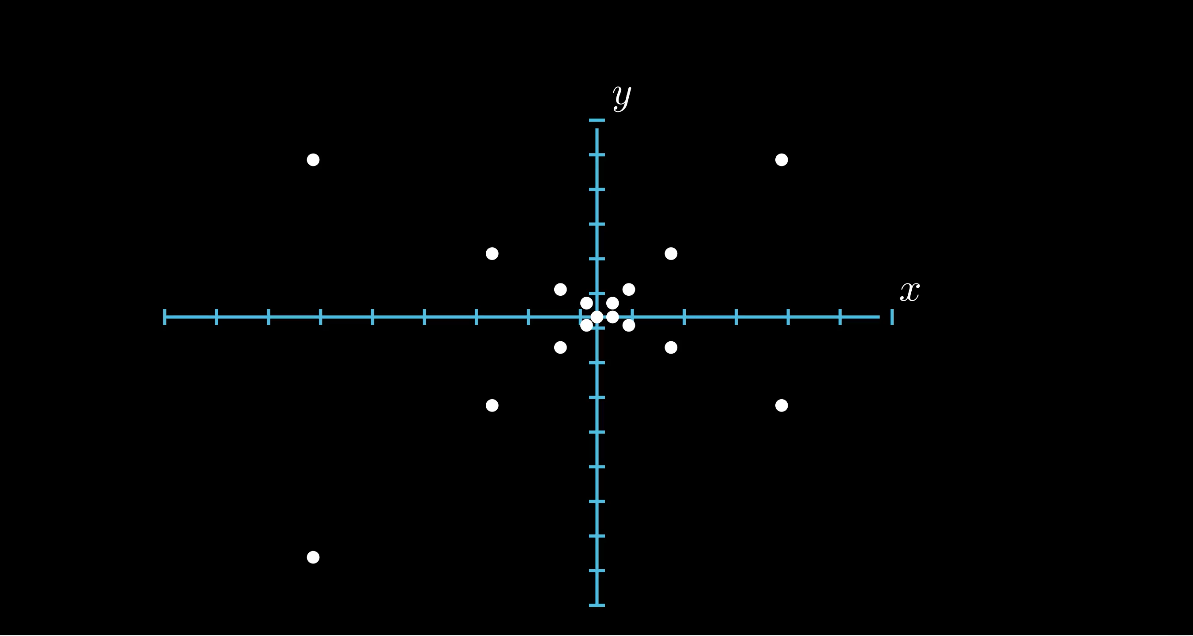
\includegraphics[scale=0.23, trim={3cm 0 6cm 0}, clip]{images/GFKT3.png}
		\caption{Plot of $P(n)$}
	\end{minipage}\hfill
	\begin{minipage}{0.45\textwidth}
		\centering
		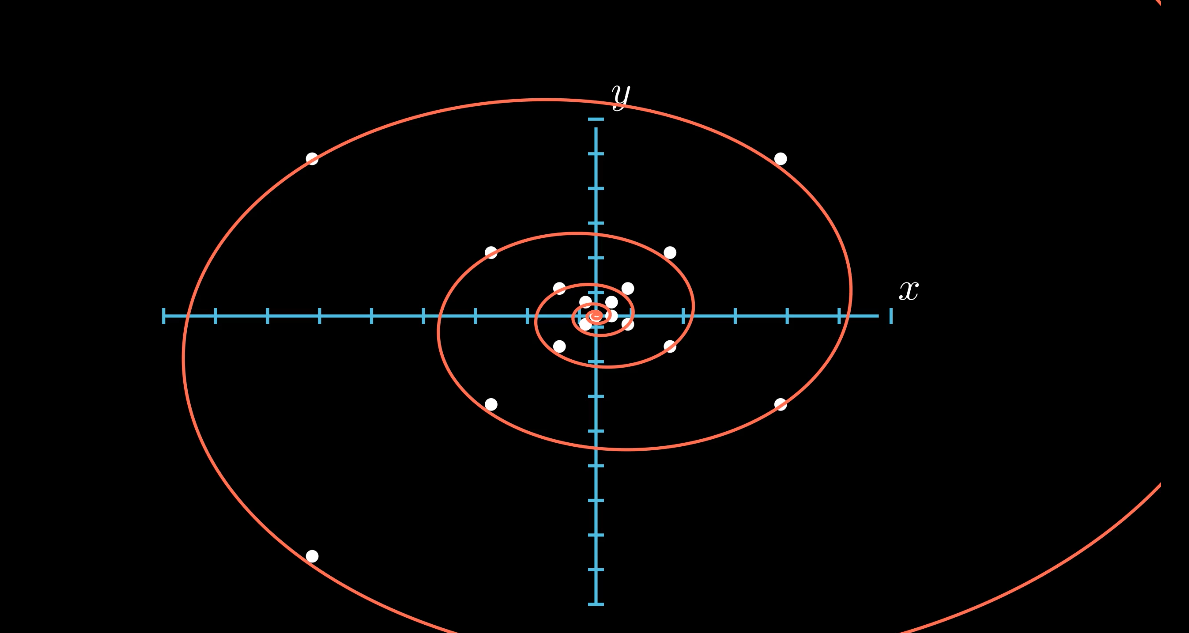
\includegraphics[scale=0.23, trim={3cm 0 6cm 0}, clip]{images/GFKT4.png}
		\caption{Logarithmic Spiral}
	\end{minipage}
\end{figure}
\begin{figure}[t]
	\label{figss}
	\centering
	\begin{minipage}{0.45\textwidth}
		\centering
		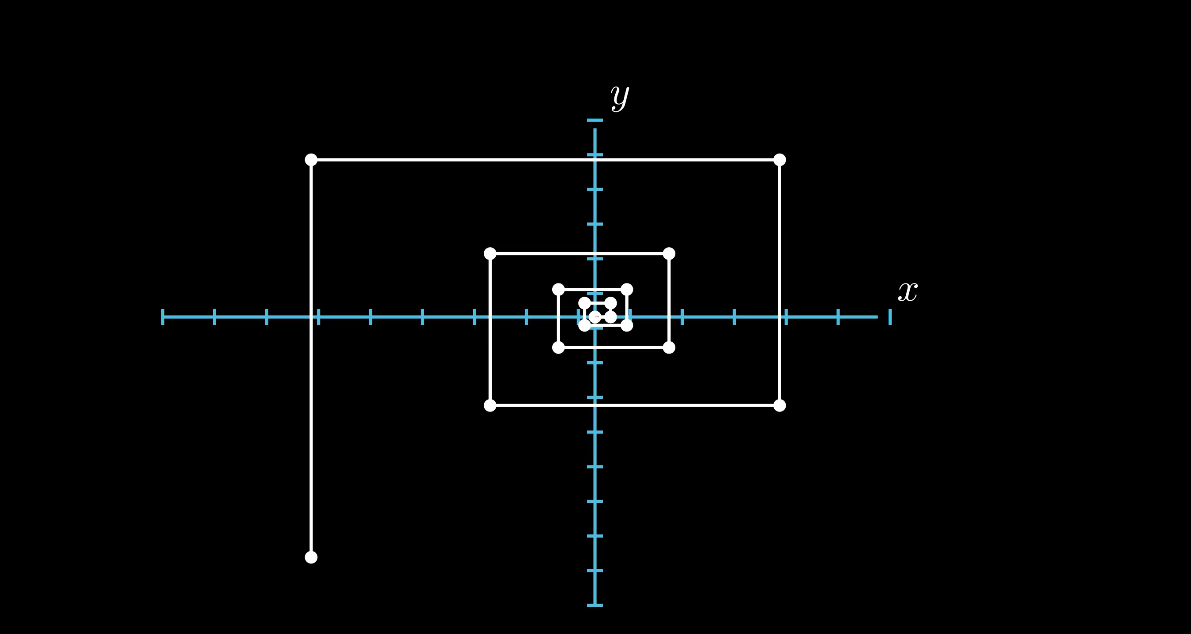
\includegraphics[scale=0.23, trim={3cm 0 6cm 0}, clip]{images/GFKT5.png}
		\caption{Plot of $L'(n)$}
	\end{minipage}\hfill
	\begin{minipage}{0.45\textwidth}
		\centering
		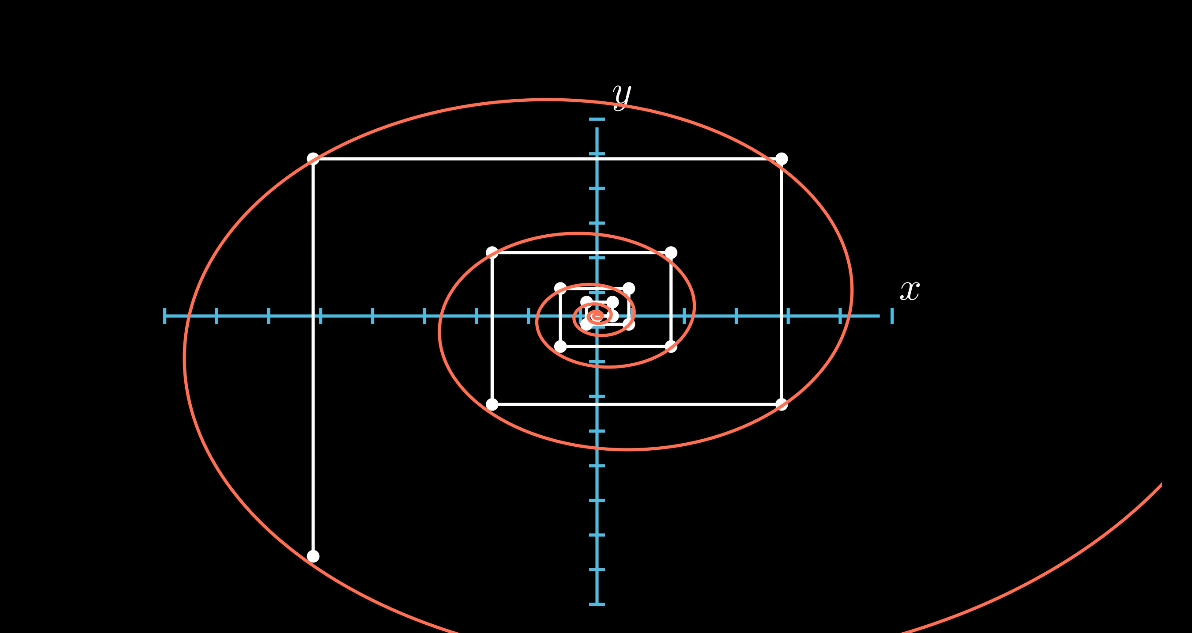
\includegraphics[scale=0.23, trim={3cm 0 6cm 0}, clip]{images/GFKT6.png}
		\caption{$L'(n)$ as discrete form of  logarithmic spiral}
	\end{minipage}
\end{figure}
\begin{figure}[t]
	\centering
	\begin{minipage}{0.45\textwidth}
		\centering
		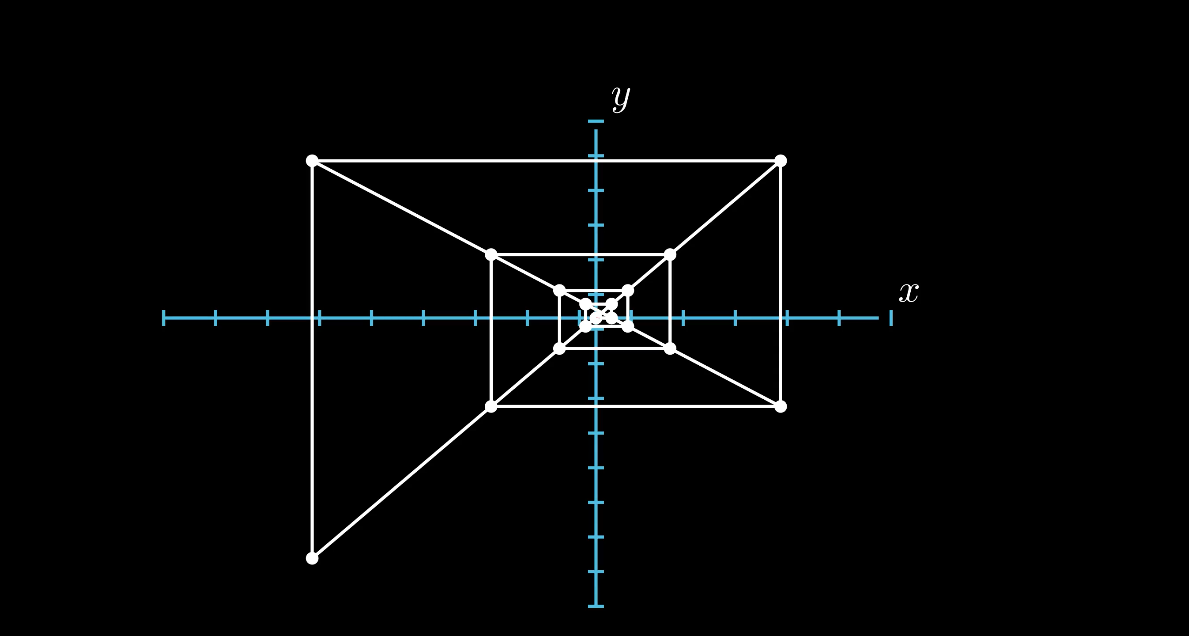
\includegraphics[scale=0.23, trim={3cm 0 6cm 0}, clip]{images/GFKT7.png}
		\caption{Plot of $T(n)$}
	\end{minipage}\hfill
	\begin{minipage}{0.45\textwidth}
		\centering
		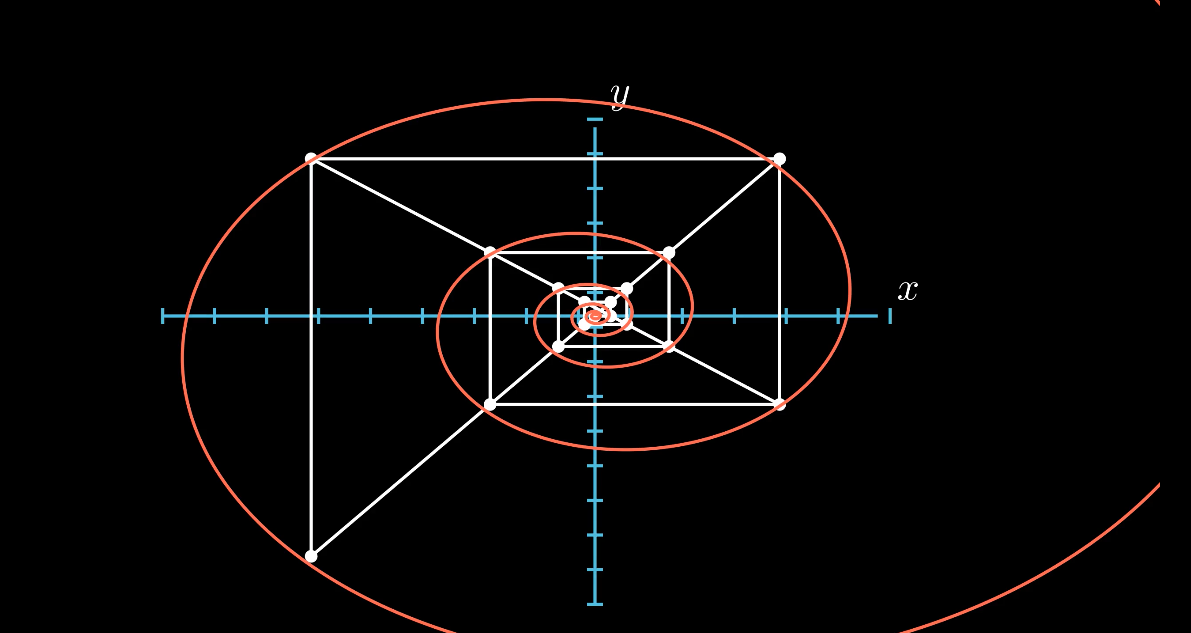
\includegraphics[scale=0.23, trim={3cm 0 6cm 0}, clip]{images/GFKT8.png}
		\caption{Complete Plot}
	\end{minipage}
\end{figure}
\clearpage
\section{Conclusion}
Thus we made use of the recurrent function $f(n) = \sqrt{f(n-1)^2 + f(n-2)^2}$,where  $f(0)$ and $f(1) \in \mathbb{R}^{+}$\\ to generate Kepler Triangles through the recurrent functions $P(n)$, $L'(n)$, $L(n)$ and\\ $T(n) = (L'(n), L'(n+1), L(n))$ at \ref{geo}, and through their geometrical arrangement obtained the logarithmic spiral {\large$$r = a\varphi^{\dfrac{\theta}{\pi}}$$}
where $a = \sqrt{\dfrac{\varphi f(1)^2 + f(0)^2}{\varphi\hspace{1mm}\sqrt{5}}}\hspace{2mm}\varphi^{-\left(\dfrac{ \tan^{-1}{\left(\sqrt{\varphi}\right)}}{\pi}\right)}$\\
We obtained $L'(n)$ as the discrete form of logarithmic spiral and for small values of $x_1$ and $y_1$ as $n \to \infty$ $P(n)$ satisfies the logarithmic spiral.

\begin{thebibliography}{9}
	
	\bibitem{paper1}
	Giuseppina Anatriello, Giovanni Vincenzi, Logarithmic Sprials and Continue triangles, Journal of Computational and Applied Mathematics, Volume 296, 2016, Pages 127-137\\ \href{https://doi.org/10.1016/j.cam.2015.09.004}{https://doi.org/10.1016/j.cam.2015.09.004}
	
	\bibitem{BF-wiki} 
	\href{https://en.wikipedia.org/wiki/Fibonacci_number#Binet's_formula}{Wikipedia Article on Fibonacci Numbers}
	
	
	\bibitem{PowerP}
	Powers of Phi by Gary Meisner,\href{https://www.goldennumber.net/powers-of-phi/}{https://www.goldennumber.net/powers-of-phi/}
	
	\bibitem{KT-wiki} 
	\href{https://en.wikipedia.org/wiki/Kepler_triangle}{Wikipedia Article on Kepler Triangles}
	
	\bibitem{LS-wiki}
	\href{https://en.wikipedia.org/wiki/Logarithmic_spiral}{Wikipedia Article on Logarithmic Spirals}
	
	\bibitem{rahulgohil2020}
	Rahul Gohil   \href{https://github.com/rahul-gohil/GFKT/releases/tag/v1.0.4}{rahul-gohil/GFKT: GFKT@1.0.4} \doi{10.5281/zenodo.3779050}
	
\end{thebibliography}

\end{document} 